\documentclass[12pt,a4paper,oneside]{memoir}
%========================================Packages============================================
\usepackage[ruled,linesnumbered]{algorithm2e}
\usepackage{graphicx}
\usepackage{subcaption}
\usepackage{titlesec}
\usepackage[left=1.25in, right=1in, top=0.75in, bottom=0.75in]{geometry}
\usepackage{setspace}
\usepackage[numbers]{natbib}
\usepackage{pdfpages}
\usepackage{titlesec}
\usepackage{xltabular}
% Set the monospaced font to Times New Roman
\usepackage{times}
\usepackage{enumitem}
\usepackage{tikz}

\usepackage{fontspec}
\setmainfont{Times New Roman}
\setmonofont{Times New Roman} 
\usepackage{listings}
\usepackage{xcolor}

\definecolor{codegreen}{rgb}{0,0.6,0}
\definecolor{codegray}{rgb}{0.5,0.5,0.5}
\definecolor{codepurple}{rgb}{0.58,0,0.82}
\definecolor{backcolour}{rgb}{0.95,0.95,0.92}


\usetikzlibrary{shapes.geometric, arrows, positioning}

\tikzstyle{block} = [rectangle, draw, fill=blue!20, 
    text width=8em, text centered, rounded corners, minimum height=4em]
\tikzstyle{line} = [draw, -latex']
\setSpacing{1.25}
\newcommand\tab[1][0.5cm]{\hspace*{#1}}
%========================================VTU GUIDELINE for chapter section and subsection============================================
\newcommand{\tit}{\fontsize{18}{22}\selectfont}
\newcommand{\chapft}{\fontsize{16}{18}\selectfont}
\newcommand{\secfnt}{\fontsize{16}{18}\selectfont}
\newcommand{\ssecfnt}{\fontsize{14}{16}\selectfont}
\newcommand{\sssecfnt}{\fontsize{12}{14}\selectfont}

\titleformat{\chapter}[display]
  {\normalfont\chapft\bfseries}{\chaptertitlename\ \thechapter}{20pt}{\tit\centering}

\titleformat{\section}
  {\normalfont\secfnt\bfseries}{\thesection}{1em}{\raggedright}

\titleformat{\subsection}
  {\normalfont\ssecfnt\bfseries}{\thesubsection}{1em}{\raggedright}

\titleformat{\subsubsection}
  {\normalfont\sssecfnt\bfseries}{\thesubsubsection}{1em}{\raggedright}
\captionsetup[figure]{labelfont={bf},textfont={bf}}
\captionsetup[table]{labelfont={bf},textfont={bf}}


\setsecheadstyle{\secfnt\bfseries\raggedright}
\setsubsecheadstyle{\ssecfnt\bfseries\raggedright}
\setsubsubsecheadstyle{\sssecfnt\bfseries\raggedright}
\setlength{\beforechapskip}{0pt} 
\setlength{\afterchapskip}{20pt} 
\setcounter{tocdepth}{2}
\setcounter{secnumdepth}{3}
\setsecnumdepth{subsection}
%Do not change anything above it
\begin{document}
%======================================Front Pages=========================================================================
\includepdf{PDFs/co1.pdf} % Make sure this path is correct

\includepdf{PDFs/co1.pdf}

\includepdf{PDFs/c3.pdf}

\includepdf{PDFs/dd1.pdf} % Make sure this path is correct

\includepdf{PDFs/5_ExecutiveSummaryAndAcknowledgement3.pdf} % Make sure this path is correct

\lstdefinestyle{mystyle}{
  basicstyle=\ttfamily,
  breaklines=true,
  showstringspaces=false,
  frame=single,
  numbers=left,
  numberstyle=\small,
  numbersep=5pt,
  xleftmargin=10pt,
  tabsize=2,
  keywordstyle=\color{blue},
  commentstyle=\color{green!50!black},
  stringstyle=\color{red}
}

\pagestyle{plain}
\pagenumbering{none}
\frontmatter
\pagenumbering{roman}
\renewcommand{\contentsname}{Table of Contents}
\tableofcontents
\newpage
\listoffigures
\newpage
\listoftables 
\mainmatter 
\pagenumbering{arabic}
%======================================Header and Footer========================
\pagestyle{myheadings}
\makeheadrule{myheadings}{\textwidth}{0.4pt}
\makefootrule{myheadings}{\textwidth}{0.4pt}{\footruleskip}
\makeoddhead{myheadings}{\small{Asthama Classification using Artificial Intelligence and Machine Learning}}{\small{\leftmark}}{\small{2024-25}} % Chnage Title and Academic Year
\makeoddfoot{myheadings}{\small{Department of Master of Computer Applications (MCA), VCET, Puttur}}{}{\small Page {\thepage}}
%======================================Chapter Starts========================
\chapter{Introduction}
By allowing systems to imitate human intellect and learn from data to make wise judgments, artificial intelligence (AI) and machine learning (ML) are game-changing technologies that have completely changed a number of sectors. I concentrated on investigating these cutting-edge technologies during my internship, especially how they may be applied to address pressing issues in the real world.\\
Gaining a thorough understanding of AI and ML principles, tools, and frameworks while using them to a particular project was the main goal of the internship. I was able to explore both the theoretical and practical facets of AI and ML through my concentration area, which included [insert specific field, such as natural language processing, predictive analytics, picture recognition, etc.].
This report highlights the goals, approaches, and results of my internship work, demonstrating how the acquired knowledge and abilities have been used to tackle the problems in the selected field.

\section{Company Profile}
With a wide range of services including Web-based development, mobile application development, graphic design, and Windows applications, Codelab Systems is a quickly growing leader in computer program implementation. Our dedication to providing innovative solutions is demonstrated by our global footprint, which includes strategic business development activities in the United Arab Emirates, Saudi Arabia, and Qatar in addition to our headquarters in Mangalore. With more than 8 years of experience in the field, Codelab Systems' goods and services are widely used.
Our greatest asset is our committed group of highly qualified specialists. Our staff, which is housed within Intellect's strong infrastructure, is highly skilled in software development and web design, using the newest technologies to produce top-notch solutions. For flawless customer experiences, we provide end-to-end services that include software development, web hosting, and domain registration. Client satisfaction is a top priority for Codelab Systems, which proactively attends to customer demands via interactive sessions during project development.
We are positioned as a reliable partner for complete IT solutions on a global basis thanks to our user-friendly products and services, which feature simple controls and excellent specifications.
To assist individuals and companies globally in reaching their greatest potential. The inspiring vision statement of Codelab is to assist individuals. As you can see, its goal isn't to do business; the focus is on people and providing them with the services they need to be their best selves.
Codelab has several initiatives aimed at achieving this goal. It strongly supports corporate responsibility, diversity, inclusivity, and environmental issues.
A group of people who collaborate is called an organization; examples include corporations, unions, charities, and neighborhood associations. The term "organization" can be used to describe a company, group, or the process of creating something. The methodical placement of human resources inside an organization to accomplish shared commercial goals is known as organizational structure (OS). It describes each employee's duties and obligations to ensure that information and work flow freely and that the organization runs smoothly.

\begin{figure}[h]
    \centering
    
\includegraphics[width=0.5\linewidth]{Images/2.png}
    \caption{Company Logo}
    \label{fig:logo}
\end{figure}

\begin{flushleft}
\textbf{Name of the Company:} CodeLab Systems \\[2pt]
\textbf{Address:} Ground Floor, Light House Condominium, \\
Light House Hill Rd, Bhavutagudda, \\
Mangalore, Karnataka 575001 \\[2pt]
\textbf{Contact Numbers:} 994518705, 7349350390 \\[2pt]
\textbf{Email:} codelabsystems@gmail.com \\[2pt]
\textbf{Website:} \ url{http://codelabsystems.in}
\end{flushleft}


\section{Functional Requirements}
Functional requirements provide the core capabilities and operations of the system and specify how it should react to various inputs or conditions. These criteria serve as the foundation for the system's design, development, and testing phases.\\
The following are the functional requirements:\\
\begin{itemize}
    \item \textbf{Data Collection and Preprocessing} \\
The system must make it easier to collect datasets from multiple sources in order to guarantee diversity and relevance to the problem domain. Additionally, it must preprocess the data, which include cleaning to remove abnormalities, normalizing numbers for uniformity, and correcting any missing or incomplete information. The correctness and suitability of the data for further processing are ensured by these methods.
    
    \item \textbf{Model Training} \\
The system should facilitate machine learning model training by utilizing suitable algorithms tailored to the project's requirements. Support must also be provided for hyperparameter tweaking, an essential process for optimizing the model's performance by changing key parameters to achieve the best results.

    \item \textbf{Prediction and Decision-Making} \\
The system must use the trained models to process new incoming data in order to generate accurate predictions. These projections, which provide useful information to stakeholders or system users, should serve as the foundation for decision-making processes.

    \item \textbf{User Interface} \\
The system's user-friendly interface should allow users to interact with the application effectively. This interface must allow users to easily enter data and view outputs utilizing detailed charts, graphs, or other analytics tools in order to increase user engagement and comprehension overall.

   \item \textbf{Real-Time Processing} \\
For circumstances requiring prompt responses, the system must handle real-time data streams. When new data is added, this ensures that the system remains responsive and current, providing users with immediate outputs or updates.

   \item \textbf{Error Handling} \\
The system should be robust in discovering and controlling mistakes or anomalies during data processing or prediction. To preserve system dependability and user confidence, clear error reporting and mitigation techniques are crucial.

   \item \textbf{Scalability and Integration} \\
To accommodate growing functionality or growing datasets without noticeably degrading performance, the system needs to be scalable. It should also seamlessly integrate with external APIs, tools, or platforms to increase its operational reach and flexibility.
\end{itemize}
When taken as a whole, these functional requirements ensure that the system can successfully manage project objectives, deliver consistent performance, and meet user expectations.

\section{Non Functional Requirements}
Rather than defining a system's capabilities, non-functional requirements specify how it should operate. They typically deal with the system's quality attributes, ensuring that it meets performance, reliability, and user satisfaction standards. The general characteristics that affect system scalability and user experience are the focus of these requirements.\\
The following are the functional requirements:\\

\begin{itemize}
    \item \textbf{Performance} \\
 The system must be able to process predictions, model training, and data input rapidly. It should be able to handle large datasets efficiently and generate predictions or insights in a timely manner. A fast response time is crucial for user satisfaction, especially in real-time applications.
    
    \item \textbf{Scalability} \\
Machine learning models should be easy to train with the system's suitable algorithms tailored to the project's requirements. The process of hyperparameter tuning, which is essential for optimizing the model's performance by changing significant parameters to achieve the best results, must also be enabled.

    \item \textbf{Reliability} \\
The system must use the trained models to process new incoming data in order to generate accurate predictions. These projections, which provide useful information to stakeholders or system users, should serve as the foundation for decision-making processes.
    \item \textbf{Usability} \\
The system's user-friendly interface should allow users to interact with the program effectively; to enhance user engagement and comprehension in general, the interface should allow users to easily enter data and view outputs using detailed charts, graphs, or other analytics tools.

   \item \textbf{Security} \\
The system must protect user data and prevent unauthorized access. Secure authentication methods and encryption should be used to safeguard the integrity and confidentiality of sensitive data.

   \item \textbf{Maintainability} \\
The system should be easy to maintain and update. It must be built with easily readable, modular code that can be easily altered to add new features or fix issues as they arise. Regular system upgrades and patches should be simple to apply.

   \item \textbf{Availability} \\
The system should be accessible and available with minimal downtime. Especially if real-time apps are being used, it must be able to run continuously so that users can use the system whenever they choose.

  \item \textbf{Compatibility} \\
The system must be compatible with a range of browsers and devices in order to allow for broad accessibility. For users to interact with it in a range of contexts, it should be interoperable with several platforms and operating systems.
\end{itemize}
These non-functional requirements ensure that the system not only performs its intended functions but also meets stringent quality, user experience, and operational efficiency requirements.

\section{Software Requirements}
Software requirements are the basic instruments, frameworks, and technologies that were used to build the project. These requirements ensure that the system is built efficiently and has the resources required to achieve its objectives. The foundation for an effective project's development, implementation, and maintenance is a well-defined set of software requirements.

\subsection{Programming Language and Frameworks}
Because of its robust machine learning and artificial intelligence modules and frameworks, Python is used to build the project. Important frameworks include TensorFlow for deep learning, scikit-learn for traditional machine learning methods, and pandas for data processing. The integration of many technologies enables the seamless building, training, and testing of models.

\subsection{Integrated Development Environment (IDE)}
An integrated development environment such as Jupyter Notebook makes it much easier to write, debug, and run code. These environments include essential features for organizing code and visualizing data, making them perfect for projects involving data-heavy processes and iterative model building.



\subsection{Frameworks and Libraries}
The software development process made use of a number of significant frameworks and libraries to enhance the system's performance and functionality:

\begin{itemize}
    \item \textbf{TensorFlow} \\
TensorFlow, a popular open-source framework for building machine learning models, was used to develop and train deep learning techniques, such as neural networks for classification and prediction tasks.
    
    \item \textbf{Scikit-learn} \\
This machine learning library was used to implement a number of traditional machine learning techniques, such as classification, regression, and clustering.

\item \textbf{Keras}\\
TensorFlow was used in combination with Keras, a high-level API for creating neural networks, to streamline the model-building procedure. Its intuitive interface made it possible to quickly design and experiment with different architectures.

    \item \textbf{Pandas} \\
Datasets were handled and cleaned using Pandas, a powerful data manipulation library, to guarantee that the data fed into machine learning models was suitably preprocessed.

    \item \textbf{NumPy} \\
NumPy made numerical calculations easier, particularly when handling large arrays and matrices, which are crucial for machine learning model training.
\end{itemize}

\subsection{
User Interface Design }
The system's user interface (UI) was designed with responsiveness, usability, and simplicity in mind to give users the greatest possible experience across a variety of devices. The frontend was primarily created using HTML, CSS, and the Flask web framework.
Libraries such as Matplotlib, Seaborn, and Plotly were utilized for data visualization and reporting in order to provide interactive visualizations, charts, and graphs that aided users in understanding the findings.

In conclusion, the technology and software tools selected had a significant impact on the project's successful development. The combination of Python programming, cloud platforms, machine learning frameworks, and security solutions resulted in a scalable, reliable, and efficient system that can handle difficult data processing tasks and deliver exceptional results. 
\chapter{System Requirements and Analysis}
\section{Introduction}
System requirements and analysis provide a comprehensive overview of the essential components needed to design, build, and maintain the system successfully. This section covers the required hardware and software, browser compatibility difficulties, UI design criteria, and security procedures to ensure that the system functions properly while maintaining user satisfaction and data security.

\section{Project Perspective}
From a project perspective, the Asthma Disease Classification Using Machine Learning system aimed to classify asthma severity levels using data-driven techniques, assisting healthcare providers in making timely and accurate diagnoses. By building a robust pipeline that comprised data collection, preprocessing, feature engineering, model training, and deployment, this project made sure the solution was scalable, user-friendly, and reliable for real-world applications. This project demonstrated how machine learning may enhance healthcare process optimization, patient care, and medical decision-making.

\section{Project Function}
The Classification of Asthma Disease Based on patient data, a machine learning system is intended to provide medical practitioners with a sophisticated, dependable tool for determining the severity of asthma. The technology offers a thorough method to help physicians diagnose asthma more precisely and effectively by utilizing potent machine learning algorithms. To ensure a diversity of inputs for classification, the system gathers a range of patient data, such as demographics, medical history, spirometry results, and symptom frequency.


The system uses extensive data preprocessing procedures to guarantee the accuracy and dependability of the predictions. Imputation techniques are used to manage missing values, and inconsistencies are removed by normalizing numerical inputs to a standard range. Techniques like one-hot encoding are used to encode categorical variables, including symptom kinds or medication history, to make sure the data is in the right format for machine learning algorithms. Key clinical characteristics are the subject of feature selection and engineering procedures, which are essential for precise asthma severity prediction.

Based on their capacity to manage intricate, high-dimensional medical data, the machine learning models used in the system—Logistic Regression, Random Forest, and Support Vector Machines (SVM)—were carefully chosen. Accuracy, precision, recall, and F1-score are among the performance indicators used to assess each algorithm once it has been trained on historical data. Clinicians can evaluate the accuracy of the outcomes by using the confidence scores that the algorithm provides for each prediction. Clinical decision-making is facilitated by the visualization of these predictions through clear, simple charts and graphs.

Additionally, the system's deployment as an intuitive online application allows for seamless integration into clinical workflows. Through a secure web interface, medical personnel can immediately enter patient data, and the system provides immediate estimates of the severity of asthma. Comprehensive insights can be used to develop reports that support treatment planning and patient care. The web-based design of the system makes it simple to access from a variety of devices, such as smartphones, tablets, and desktop computers, enhancing the availability of vital diagnostic data across a range of healthcare environments.

Because the system manages sensitive patient data, security is a key component of the architecture. To protect patient privacy, all data exchanges are encrypted, and access control measures are put in place to guarantee that only individuals with the proper authorization can access and handle the data. To adhere to medical data regulations, regular security audits are conducted, guaranteeing the system's continued security and reliability.

In conclusion, by offering precise forecasts, real-time decision assistance, and secure data handling, the Asthma Disease Classification Using Machine Learning system not only improves the diagnostic skills of medical professionals but also raises the general effectiveness of asthma management. The system's user-friendly design and scalable architecture guarantee practical utility in actual medical settings, improving asthma treatment and results.



\section{General Constraint}
The limitations and conditions that must be taken into account when developing and implementing a system are referred to as general constraints. These restrictions ensure that the system operates effectively in the specified environment. Common constraints include hardware limitations that impact system performance, such as processor power, memory, or storage capacity. Additionally, software compatibility with specific operating systems or development tools may limit functionality. Time and resource constraints, including tight deadlines or budgetary constraints, may also have an effect on the project's scope. Additional restrictions may be imposed by legal and compliance requirements to safeguard data security and privacy, particularly in sensitive sectors like healthcare or finance. To provide a system that is scalable, dependable, and functional, these limitations must be recognized and addressed.
One of the main elements influencing a system's performance is frequently its hardware limitations. Particularly when working with big datasets or real-time processing, the hardware's processing power, memory, and storage capacity must be adequate to meet the application's computing demands. In the case of machine learning models, for example, insufficient hardware resources may lead to long training times, unsatisfactory model performance, or even system crashes. Delivering a high-performance application requires optimizing the system to function efficiently within the specified hardware constraints.
On the software side, limitations pertaining to the system's interoperability with particular operating systems or development platforms are frequently encountered. It may be necessary to modify the program or use certain libraries or frameworks in order for it to function flawlessly with the platforms and operating systems that end users will use. Furthermore, certain systems can be dependent on proprietary software or certain development tools, which could result in restrictions on their scalability, integration, or usefulness.

\section{Requirements}
\subsection{Hardware Requirements}The complexity of the system, including the amount of data it processes, the number of users accessing it at once, and the type of tasks it completes—especially for data analysis and machine learning—determines the hardware needs. The recommended hardware specifications are as follows:

\begin{itemize}
\item \textbf{Processor:} Minimum of Intel i5 or equivalent.
\item \textbf{RAM:} At least 4 GB for basic operations; 8 GB or more for smooth multitasking.
\item \textbf{Storage:} 2 GB of free disk space for browser-based usage and temporary storage.
\item \textbf{Browser Compatibility:} Browser-based and compatible with modern web browsers like Chrome, Firefox, Safari, or Edge.
\end{itemize}

\subsection{Software Requirements}
Supporting the system's development, implementation, and operation depends heavily on the software requirements. The platforms, frameworks, and tools listed below were utilized:

\begin{itemize}
\item \textbf{Operating System:} Windows 8 and above
\item \textbf{Code Language:} Python
\item \textbf{Tools:} Anaconda
\item \textbf{Editor:} Jupyter Notebook
\item \textbf{Libraries:} Numpy, pandas, sklearn, matplotlib, pickle, etc.
\end{itemize}

\section{Design}
To guarantee data integrity, model dependability, and defense against malevolent attacks, AI and ML systems need strong security measures. A condensed overview of important security procedures is provided below:


\begin{figure}[h]
\centering
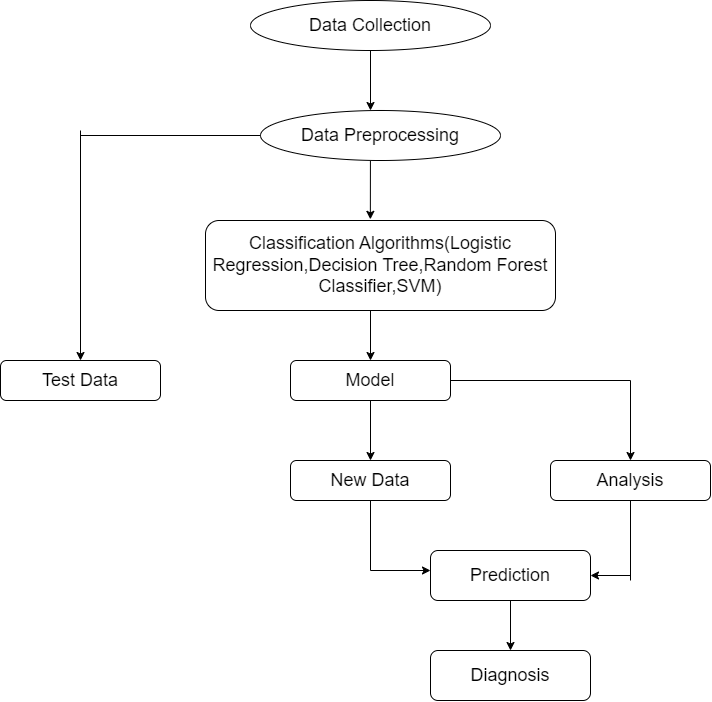
\includegraphics[width=0.7\linewidth]{Images/cc.png}
\caption{Context Flow Diagram}
\label{fig:enter-label}
\end{figure}

\begin{figure}[h]
\centering
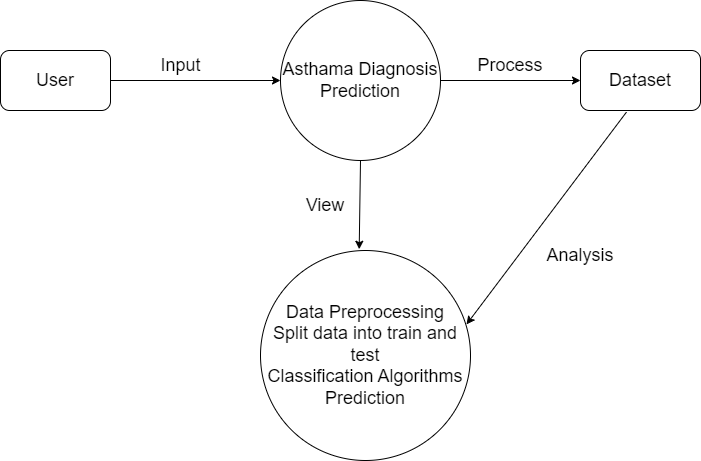
\includegraphics[width=0.7\linewidth]{Images/dd.png}
\caption{Data Flow Diagram}
\label{fig:enter-label}
\end{figure}
Data collection is a component of the asthma categorization system that entails gathering patient information such as demographics, symptoms, and medical history. To guarantee consistency, this raw data is cleaned and encoded during the data preprocessing step. The likelihood of asthma is then predicted using a variety of classification algorithms (such as SVM, Random Forest, Decision Tree, and Logistic Regression). The model processes fresh inputs to produce a prediction once its accuracy has been tested using different data. To guarantee a trustworthy diagnosis and assist well-informed healthcare decisions, the results are verified and examined.


The user, dataset, and processing components interact in the asthma diagnostic prediction system. A preloaded dataset containing patient data is used to process user inputs, such as symptoms. By separating data into training and testing sets, the system carries out data preprocessing. Predictions are produced using machine learning classification algorithms. An accurate diagnosis of asthma is aided by the analysis and display of these results to the user.

\chapter{Project Carried Out}

\section{Introduction}
Millions of people worldwide suffer from asthma, a chronic respiratory disease. Breathing becomes difficult as a result of episodes of airway inflammation and constriction. For asthma to be effectively managed and treated, severity classification must be done accurately. Conventional diagnostic techniques, such as subjective evaluations and physical exams, might not be as accurate as they need to be for the best possible treatment planning.

The goal of this study is to utilize machine learning (ML) to categorize asthma severity levels using patient data. Our goal is to create a system that improves diagnostic precision, permits prompt treatments, and aids medical professionals in making well-informed decisions by employing a data-driven approach. The system predicts the severity of asthma and provides accurate treatment recommendations by analyzing a number of variables, such as patient demographics, medical history, spirometry findings, and symptom frequency.

To guarantee strong classification performance, the suggested system incorporates a variety of machine learning methods, including Random Forest, Support Vector Machines (SVM), and Logistic Regression. The method saves diagnostic time and human error by automating the prediction process, which eventually improves asthma management and patient outcomes.

\subsection{Motivation}
The increasing incidence of asthma and the difficulties medical professionals encounter in properly diagnosing and treating the condition are the driving forces behind this research. Determining the best course of treatment requires an accurate and rapid classification of asthma severity, but traditional diagnostic techniques frequently rely on manual patient data interpretation and subjective clinical assessments.

As electronic health records (EHRs) become more widely available and medical data volumes increase, machine learning presents a chance to transform asthma diagnosis through the use of unbiased, data-driven insights. Healthcare professionals can give patients with better individualized care by receiving quick, accurate, and trustworthy forecasts by automating the asthma classification process.

Furthermore, a major driving force behind this effort is the possibility that machine learning may continue to advance over time as a result of exposure to fresh data and feedback. Asthma sufferers' quality of life may increase as a result of more efficient asthma management techniques brought about by the system's capacity to adjust and improve its accuracy.

\subsection{Methodology}
A methodical procedure was used to create the Asthma Disease Classification System. To guarantee consistency and quality, patient data was gathered and preprocessed, including demographic information, medical history, and clinical test results. To categorize the severity of asthma, machine learning algorithms including Support Vector Machines, Random Forest, and Logistic Regression were trained using historical patient data. Reliability was ensured by evaluating the models using accuracy and F1-score. In the end, the system was implemented as a safe and intuitive web application that protected patient data while giving medical experts real-time forecasts.
\subsection{Outcomes}
Asthma severity levels were accurately defined using the Asthma Disease Classification System, allowing for prompt and accurate diagnosis. By lowering manual errors and improving healthcare workers' decision-making, the use of machine learning models increased diagnostic precision. Clinical operations were eased by the intuitive web application, which offered thorough insights and real-time forecasts. Sensitive patient data was also protected by strong security measures, which made the system reliable and efficient for everyday use.

\section{Codes}
\subsection{Import Data}
\begin{verbatim}
import pandas as pd
import numpy as np
import matplotlib.pyplot as plt
df=pd.read_csv(r"C:\Users\varun\Downloads\asthma_disease_data.csv")
df
\end{verbatim}
\subsection{Data Columns and Shape}
\begin{verbatim}
df.columns
Output:Index(['PatientID', 'Age', 'Gender', 'Ethnicity', 
'EducationLevel', 'BMI', 'Smoking', 'PhysicalActivity', 
'DietQuality', 'SleepQuality','PollutionExposure', 
'PollenExposure', 'DustExposure', 'PetAllergy',
'FamilyHistoryAsthma', 'HistoryOfAllergies',
 'Eczema', 'HayFever','GastroesophagealReflux',
 'LungFunctionFEV1', 'LungFunctionFVC', 'Wheezing', 
'ShortnessOfBreath', 'ChestTightness', 'Coughing',
'NighttimeSymptoms', 'ExerciseInduced',
 'Diagnosis', 'DoctorInCharge'],dtype='object')
df.shape
(2392, 29)
\end{verbatim}
\subsection{Visualization}
\subsubsection{Gender Distribution (Bar Chart)}
\begin{verbatim}
df['Gender'].unique()
gen=df['Gender'].value_counts()
x=gen.index
y=gen.values
plt.figure(figsize=(6,4))
plt.title('Gender Distribution')
plt.bar(x,y,color=['black','pink','red'])
plt.xlabel('Gender')
plt.ylabel('Counts')
plt.show()
\end{verbatim}

\textbf{Ouput:}
\begin{figure}[h]
\centering
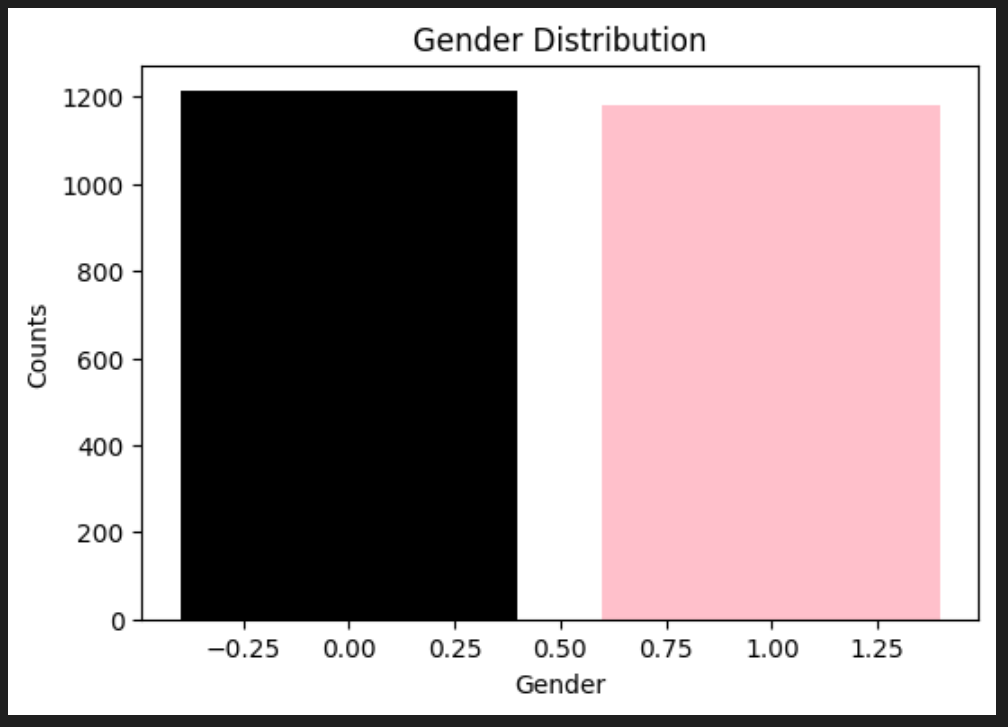
\includegraphics[width=0.7\linewidth]{Images/1.png}
\caption{Bar chart}
\label{fig:enter-label}
\end{figure}
The gender distribution in the dataset is displayed in the first figure using a bar chart. The number of individuals is displayed on the y-axis, while gender is displayed on the x-axis. The black bar most likely represents the male gender category, whereas the pink bar most likely represents the female gender category. The figure demonstrates that the counts are almost similar for both genders, with a little higher count in the pink category. Since the gender axis labels (such as 0 and 1) are not obvious, it would be helpful to specifically designate the categories (such as "Male" and "Female") for easier comprehension.

\subsubsection{Education Level Distribution (Pie Chart)}
\begin{verbatim}
df['EducationLevel'].unique()
edu=df['EducationLevel'].value_counts()
x=edu.index
y=edu.values
plt.figure(figsize=(6,4))
plt.title('Education Level Distribution')
plt.pie(y,labels=x)
plt.legend(x,loc="upper right")
plt.show()
\end{verbatim}

\textbf{Ouput:}
\begin{figure}[h]
\centering
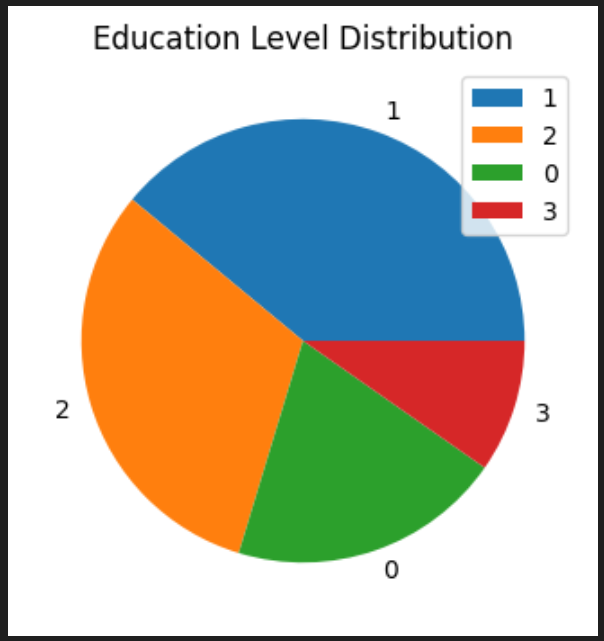
\includegraphics[width=0.7\linewidth]{Images/g2.png}
\caption{Pie Chart}
\label{fig:enter-label}
\end{figure}
The subsequent graphic uses a pie chart to display the distribution of education levels within the dataset. The legend states that each component stands for a different educational level: Red is represented by three, orange by two, and green by zero. Education levels "0" (green) and "3" (red) have lesser proportions than levels "1" (blue) and "2" (orange), according to the chart. This suggests that most people in the dataset have intermediate education levels (represented by 1 and 2), but basic (0) and higher education (3) levels are less prevalent. The distribution's obvious legend and markings make it simple to understand.

\subsubsection{ Age Distribution (Histogram)}
\begin{verbatim}
df['Age'].min()
df['Age'].max()
x=df['Age']
plt.figure(figsize=(8,6))
plt.title('Age Distribution')
plt.hist(x,bins=[10,20,30,40,50,60,70,80],color='yellow')
plt.xlabel('Age')
plt.ylabel('Counts')
plt.show()
\end{verbatim}
\textbf{Ouput:}
\begin{figure}[h]
\centering
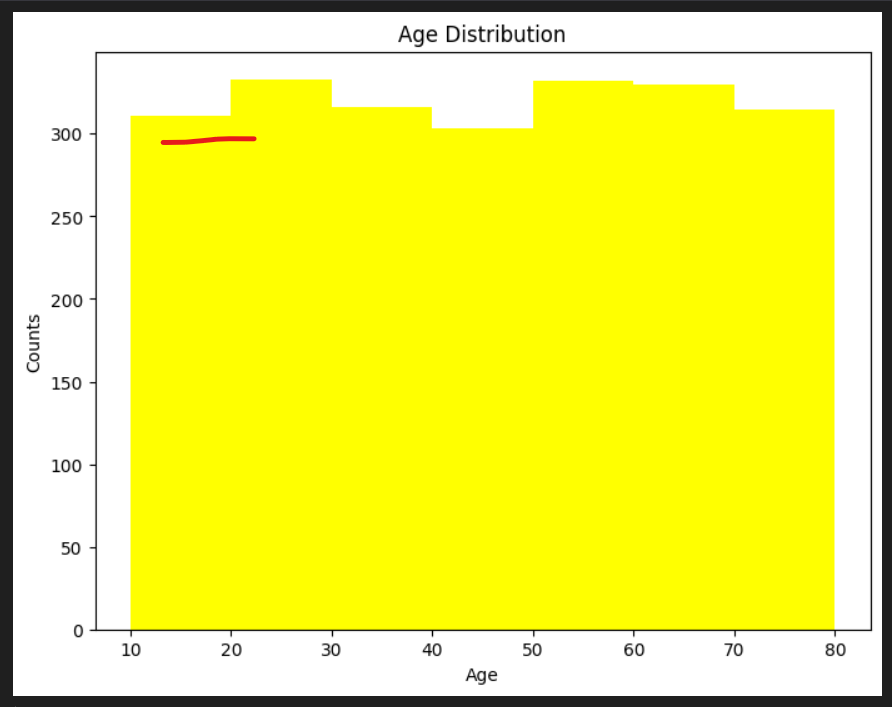
\includegraphics[width=0.7\linewidth]{Images/g1.png}
\caption{Histogram}
\label{fig:enter-label}
\end{figure}
 displays the age distribution of individuals using a histogram. The x-axis displays the age range, and the y-axis displays the number of individuals in each age bin. The data appears to be evenly distributed across the age range (10 to 80 years), as most bins contain almost equal numbers (approximately 300 people). This suggests that different age groups are fairly represented in the sample. Even while the bright yellow of the bars makes them visible, choosing a less bright tint might improve their aesthetic appeal. Adding more thorough age bin labels on the x-axis would further increase readability.

\subsection{Splitting Data}
\begin{verbatim}
from sklearn.model_selection import train_test_split
x_train,x_test,y_train,
y_test=train_test_split(x,y,test_size=0.2,random_state=42)
x_test.shape
x_train.shape
y_train.shape
y_test.shape
\end{verbatim}

\subsection{LogisticRegression Algorithm}
\begin{verbatim}
from sklearn.linear_model import LogisticRegression
from sklearn.metrics import accuracy_score,confusion_matrix
from sklearn.preprocessing import StandardScaler
import seaborn as sns
lr=LogisticRegression()
lr.fit(x_train,y_train)
predict_lr=lr.predict(x_test)
predict_lr
accuracy=accuracy_score(y_test,predict_lr)
accuracy
cm=confusion_matrix(y_test,predict_lr)
cm
y_test
sc= StandardScaler()
x_train=sc.fit_transform(x_train)
x_test=sc.transform(x_test)
x_train
x_test
train_score=lr.score(x_train,y_train)
train_score
train_score=lr.score(x_test,y_test)
train_score
plt.figure(figsize=(8,4))
plt.title('confusion matricx')
sns.heatmap(cm,annot=True,fmt='d')
plt.xlabel('True value')
plt.ylabel('predicted value')
plt.show()
\end{verbatim}
\textbf{Ouput:}
\begin{figure}[h]
\centering
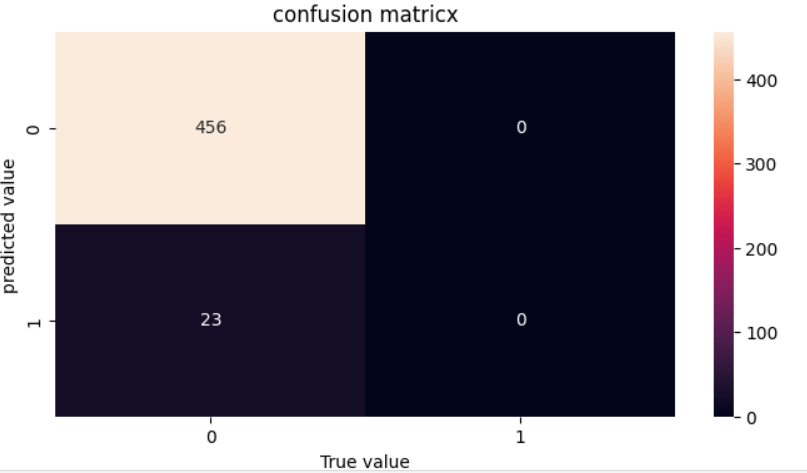
\includegraphics[width=0.7\linewidth]{Images/r1.png}
\caption{HeatMap(LogisticRegression Algorithm)}
\label{fig:enter-label}
\end{figure}
By correctly identifying 456 non-asthma cases but failing to predict any asthma cases, with 23 false negatives and no true positives, the confusion matrix assesses the model's performance in predicting asthma. This suggests that the model is biased towards predicting "No Asthma" and has trouble identifying actual asthma cases, most likely as a result of class imbalance or insufficient sensitivity.

\subsection{DecisionTreeClassifier Algorithm}
\begin{verbatim}
from sklearn.tree import DecisionTreeClassifier
from sklearn.metrics import accuracy_score,confusion_matrix
import seaborn as sns
dcl=DecisionTreeClassifier()
dcl.fit(x_train,y_train)
predict_dcl=dcl.predict(x_test)
predict_dcl
accuracy=accuracy_score(y_test,predict_dcl)
accuracy
cm=confusion_matrix(y_test,predict_dcl)
cm
y_test
train_score=dcl.score(x_train,y_train)
train_score
train_score=dcl.score(x_test,y_test)
train_score
plt.figure(figsize=(8,4))
plt.title('confusion matricx')
sns.heatmap(cm,annot=True,fmt='d')
plt.xlabel('True value')
plt.ylabel('predicted value')
plt.show()
\end{verbatim}
\textbf{Ouput:}
\begin{figure}[h]
\centering
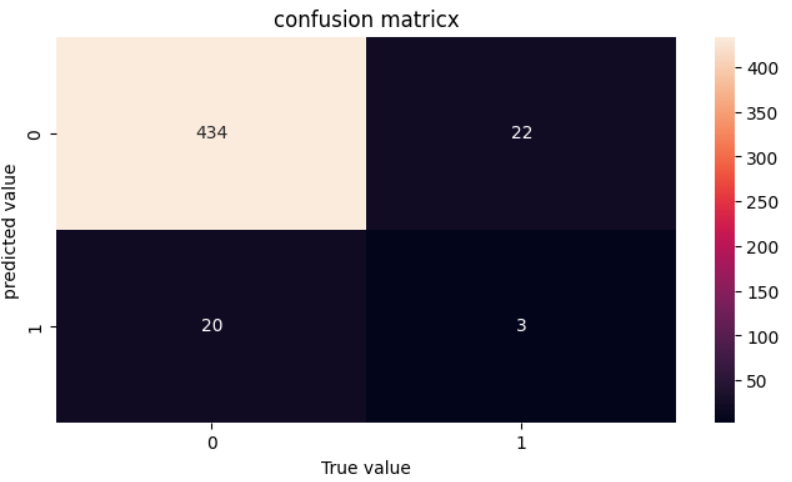
\includegraphics[width=0.7\linewidth]{Images/r3.png}
\caption{HeatMap(DecisionTreeClassifier Algorithm)}
\label{fig:enter-label}
\end{figure}
The confusion matrix demonstrates that while the model successfully predicts 434 non-asthma cases, it has trouble detecting asthma, correctly categorizing 20 asthma cases as non-asthma and only detecting three true positives. Furthermore, it misclassifies 22 occurrences of non-asthma as asthma, suggesting an imbalance between sensitivity and precision.\textbf{Above all algorithm Decision Tree Classifier give more accurate result}.

\subsection{RandomForestClassifier Algorithm}
\begin{verbatim}
from sklearn.ensemble import RandomForestClassifier
import seaborn as sns
rn=RandomForestClassifier()
rn.fit(x_train,y_train)
predict_rn=rn.predict(x_test)
predict_rn
y_test
accuracy=accuracy_score(y_test,predict_rn)
accuracy
cm=confusion_matrix(y_test,predict_rn)
cm
train_score=rn.score(x_train,y_train)
train_score
train_score=rn.score(x_test,y_test)
train_score
plt.figure(figsize=(8,4))
plt.title('confusion matricx')
sns.heatmap(cm,annot=True,fmt='d')
plt.xlabel('True value')
plt.ylabel('predicted value')
plt.show()
\end{verbatim}
\textbf{Ouput:}
\begin{figure}[h]
\centering
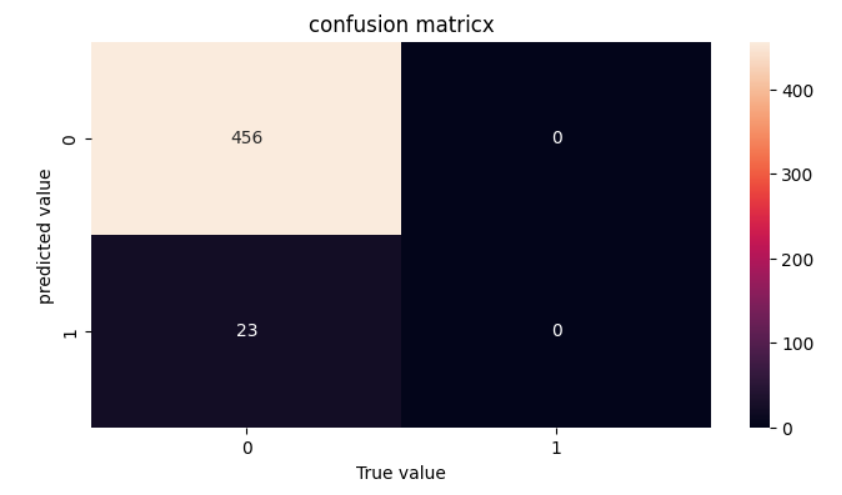
\includegraphics[width=0.7\linewidth]{Images/r2.png}
\caption{HeatMap(RandomForestClassifier Algorithm)}
\label{fig:enter-label}
\end{figure}
The confusion matrix evaluates how well the model predicts asthma. It shows that although the model correctly identifies 456 non-asthma cases, it cannot predict any asthma patients, as evidenced by the 23 false negatives and the lack of true positives. This implies that the model is biased toward predicting "No Asthma" and struggles to identify actual asthma patients, most likely due to class imbalance or low sensitivity.

\subsection{SVC Algorithm}
\begin{verbatim}
from sklearn.svm import SVC
import seaborn as sns
sc=SVC()
sc.fit(x_train,y_train)
predict_sc=sc.predict(x_test)
predict_sc
y_test
accuracy=accuracy_score(y_test,predict_sc)
accuracy
cm=confusion_matrix(y_test,predict_sc)
cm
df.isna().sum()
df.info()
plt.figure(figsize=(8,4))
plt.title('confusion matricx')
sns.heatmap(cm,annot=True,fmt='d')
plt.xlabel('True value')
plt.ylabel('predicted value')
plt.show()
\end{verbatim}
\begin{figure}[h]
\centering
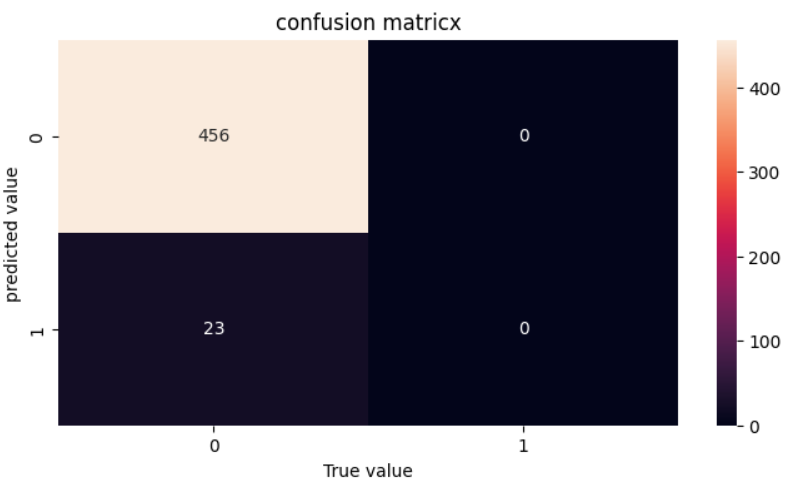
\includegraphics[width=0.7\linewidth]{Images/r4.png}
\caption{HeatMap(SVC Algorithm)}
\label{fig:enter-label}
\textbf{Ouput:}
\end{figure}
The model's asthma prediction accuracy is evaluated by the confusion matrix. It shows that although the model correctly identifies 456 non-asthma cases, it cannot predict any asthma patients, resulting in 23 false negatives and no true positives.

\subsection{Main File}
\begin{verbatim}
from flask import Flask, render_template, request
import pandas as pd
import pickle

# Load the pre-trained model
with open('a_model.pkl', 'rb') as model_file:
    model = pickle.load(model_file)

# Load the pre-trained scaler (used during training)
with open('nr_model.pkl', 'rb') as scaler_file:
    scaler = pickle.load(scaler_file)

# Initialize Flask app
app = Flask(__name__)

# Define the input features for the model
input_columns = [
    'Age', 'Gender', 'BMI', 'Smoking', 
    'PhysicalActivity', 'DietQuality', 'SleepQuality',
    'FamilyHistoryAsthma', 'LungFunctionFEV1',
     'LungFunctionFVC', 'Wheezing','ShortnessOfBreath'
]
# Route to display the form and handle user input
@app.route("/", methods=["GET", "POST"])
def index():    
    if request.method == "POST":
        # Extract the user input data
        user_input = {
            'Age': int(request.form['Age']),
            'Gender': request.form['Gender'],
            'BMI': float(request.form['BMI']),
            'Smoking': request.form['Smoking'],
            'PhysicalActivity': request.form['PhysicalActivity'],
            'DietQuality': request.form['DietQuality'],
            'SleepQuality': request.form['SleepQuality'],
            'FamilyHistoryAsthma':request.form['FamilyHistoryAsthma'],
            'LungFunctionFEV1':float(request.form['LungFunctionFEV1']),
            'LungFunctionFVC':float(request.form['LungFunctionFVC']),
            'Wheezing':request.form['Wheezing'],
            'ShortnessOfBreath':request.form['ShortnessOfBreath']
        }
        # Convert user input into a DataFrame
        input_df = pd.DataFrame([user_input])

        # Scale the input data using the pre-trained scaler
        input_scaled = scaler.transform(input_df[input_columns])

        # Make prediction
        prediction = model.predict(input_scaled)

        # Display prediction result
        diagnosis = 'Asthma' if prediction[0] == 1 else 'No Asthma'

        return render_template('result.html', diagnosis=diagnosis)
    return render_template("index.html")
@app.route('/about')
def about():
    return render_template('about.html')    

# Run the app
if __name__ == "__main__":
    app.run(debug=True)

\end{verbatim}

\subsection{index.html}
\begin{verbatim}
<!DOCTYPE html>
<html lang="en">
<head>
<meta charset="UTF-8">
<meta name="viewport" content="width=device-width, initial-scale=1.0">
<title>Asthma Prediction</title>
</head>
<body>
    <!-- Navbar -->
    <div class="navbar">
        <div class="logo">
            <h1>Asthma Prediction</h1>
        </div>
        <div class="nav-links">
            <a href="#">Prediction</a>
            <a href="{{ url_for('about') }}">Visualization</a>
        </div>
    </div>
    <!-- Main content -->
    <div class="container">
        <!-- Information about the page -->
        <div class="info">
            <h2>Welcome to the Asthma Prediction Tool</h2>
            <p>Our tool uses advanced machine learning models 
            your health data and predict whether you may have asthma. 
            Fill in the form below to get started!</p>
        </div>
        <!-- Form -->
<form method="POST">
  <label for="Age">Age:</label>
  <input type="number" id="Age" name="Age" required>

  <label for="Gender">Gender (Male/Female):</label>
  <input type="text" id="Gender" name="Gender" required>

  <label for="BMI">BMI:</label>
  <input type="number" step="any" id="BMI" name="BMI" required>

  <label for="Smoking">Smoking (Yes/No):</label>
  <input type="text" id="Smoking" name="Smoking" required>

  <label for="PhysicalActivity">Physical Activity (Yes/No):</label>
  <input type="text" id="PhysicalActivity" 
   name="PhysicalActivity" required>

  <label for="DietQuality">Diet Quality (Good/Fair/Poor):</label>
  <input type="text" id="DietQuality" name="DietQuality" required>

  <label for="SleepQuality">Sleep Quality (Good/Fair/Poor):</label>
  <input type="text" id="SleepQuality" name="SleepQuality" required>

  <label for="FamilyHistoryAsthma">Family History of Asthma (Yes/No):
  </label>
  <input type="text" id="FamilyHistoryAsthma" 
   name="FamilyHistoryAsthma" required>

  <label for="LungFunctionFEV1">Lung Function FEV1:</label>
  <input type="number" step="any" id="LungFunctionFEV1"
   name="LungFunctionFEV1" required>

   <label for="LungFunctionFVC">Lung Function FVC:</label>
   <input type="number" step="any" id="LungFunctionFVC"
    name="LungFunctionFVC" required>

   <label for="Wheezing">Wheezing (Yes/No):</label>
   <input type="text" id="Wheezing" name="Wheezing" required>

   <label for="ShortnessOfBreath">Shortness of Breath (Yes/No):</label>
   <input type="text" id="ShortnessOfBreath"
    name="ShortnessOfBreath" required>
   <input type="submit" value="Predict">
 </form>
</div>
</body>
</html>
\end{verbatim}



\chapter{Assessment and Conclusion}
\section{Project Assessment}
\begin{figure}[h]
    \centering
    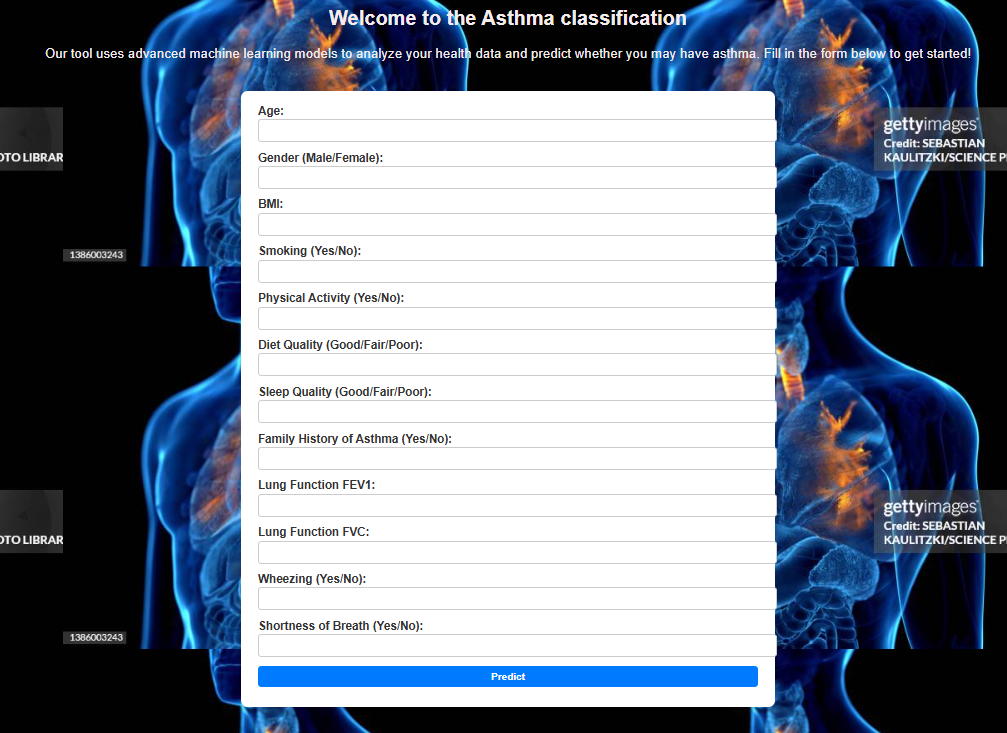
\includegraphics[width=0.9\linewidth]{Images/u1.png}
    \caption{Home Page}
    \label{fig:ui1}
\end{figure}
The asthma prediction tool starts on the Input Page, where users must enter their health-related data. Among the information in this data that helps the model understand the user's general health profile are age, gender, and BMI. Other factors, such smoking status and physical activity levels, are included since they may have an impact on respiratory health. The questionnaire also gathers information on food and sleep quality, both of which have been linked to overall lung health. The asthma prediction tool starts on the Input Page, where users must enter their health-related data. Among the information in this data that helps the model understand the user's general health profile are age, gender, and BMI. Other factors, such smoking status and physical activity levels, are included since they may have an impact on respiratory health. The questionnaire also gathers information on food and sleep quality, both of which have been linked to overall lung health. 
\begin{figure}[h]
    \centering
    \begin{minipage}{0.5\linewidth}
        \centering
        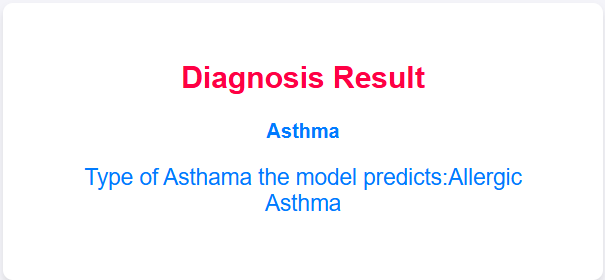
\includegraphics[width=\linewidth]{Images/u2.png}
        \caption{Allergic Asthma}
        \label{fig:ui5}
    \end{minipage}
\end{figure}
\newline
As Figure 4.2 shows that the diagnosis result indicates Asthma, specifically the type predicted by the model is Allergic Asthma.
\begin{figure}[h]
    \centering
    \begin{minipage}{0.5\linewidth}
        \centering
        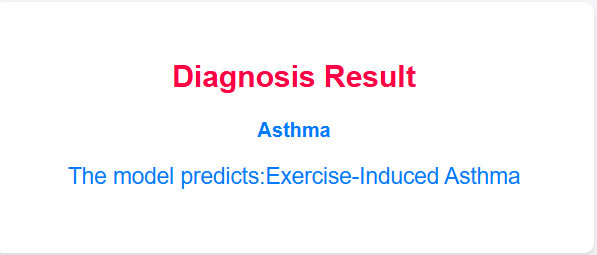
\includegraphics[width=\linewidth]{Images/u3.png}
        \caption{Exercise-Induced Asthma}
        \label{fig:ui5}
    \end{minipage}
\end{figure}
\newline 
As Figure 4.3 shows that the diagnosis result indicates Asthma, with the model predicting Exercise-Induced Asthma.
\begin{figure}[h]
    \centering
    \begin{minipage}{0.5\linewidth}
        \centering
        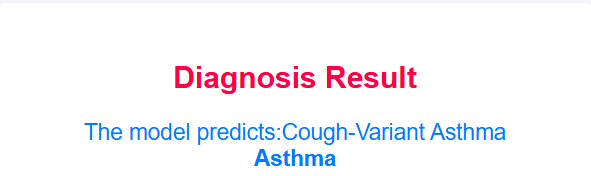
\includegraphics[width=\linewidth]{Images/u4.png}
        \caption{Cough-Variant Asthma}
        \label{fig:ui5}
    \end{minipage}
\end{figure}
\newline 
As Figure 4.4 shows that the diagnosis result indicates Asthma, and the model predicts the subtype as Cough-Variant Asthma.

\section{Personal Development}
The classification of asthma diseases was the main emphasis of the internship. By promoting technical proficiency, strengthening problem-solving abilities, and developing critical soft skills, machine learning greatly aided in human growth. Hands-on expertise with a variety of techniques, such as Support Vector Machines, Random Forest, and Logistic Regression, was made possible by participating in real-world machine learning projects. Additionally, this work involved statistical analysis, feature engineering, and advanced data preprocessing, which strengthened mastery of tools like Pandas, NumPy, and Scikit-learn. Working with frameworks like Flask also made it possible to create web-based apps for implementing machine learning models, which helped to close the gap between theory and practice.

Through challenges including managing inconsistent data, maximizing model performance, and guaranteeing system scalability, the internship honed problem-solving abilities. The exercise highlighted the need of analytical thinking and flexibility in practical situations by critically analyzing several algorithms and choosing the best one for classifying asthma.

Collaboration and time management were essential components of this experience. While regular interactions with mentors and team members enhanced collaboration and teamwork, juggling multiple tasks under short deadlines sharpened organizational skills. Additionally, communicating findings in an understandable manner through reports and visualizations improved communication skills and made complicated information understandable to both technical and non-technical audiences.
\section{Skills Consolidation}
Through weekly tasks and learning opportunities, skill in data processing, model building, and system integration rapidly developed, and significant knowledge of software development methodologies, machine learning, and artificial intelligence was acquired throughout the internship.
\begin{table}[h]
    \centering
    \caption{Week-wise Work Progress}
    \begin{center}  
        \begin{tabular}{|c|p{12.4cm}|}
            \hline
            \textbf{Week} & \textbf{Work Progress} \\ \hline
            1 &Identified the issue statement, gathered requirements, and set project objectives. Conducted a feasibility analysis to finalize the scope. \\ \hline
            2 & gathered a variety of datasets from different sources and conducted preliminary research to comprehend their structure and possible problems. \\ \hline
            3 & Datasets were cleaned, preprocessed, and divided into subsets for testing, validation, and training. Missing values and inconsistencies were fixed, and data was normalized for consistency. \\ \hline
            4 & Designed and trained the machine learning model, fine-tuning its architecture to optimize performance based on project requirements. \\ \hline
            5 & Integrated the ML model into a web application using Flask for the backend and HTML/CSS for the front end. Conducted extensive system testing to identify and resolve bugs.\\ \hline
            6 & Deployed the application, collected user feedback, and implemented final optimizations. Completed documentation and prepared the final project report. \\ \hline
        \end{tabular}
    \end{center}
    \label{tab:work}
\end{table}
\section{Conclusion}
From understanding the project objectives to putting a functional application into practice, every stage of the internship provided new insights and chances to learn new skills. Accuracy and adaptability are crucial in real-world scenarios, as demonstrated by the systematic approach to problem-solving that involved data pretreatment, model training, and system integration.\\
The final result, a successfully deployed AI/ML system, demonstrated how theoretical understanding might be applied to practical issues. It also underlined how important critical thinking, cooperation, and lifelong learning are to achieving project objectives. This internship not only improved technical skills but also promoted a deeper understanding of the complexities and potential applications of AI/ML technology in solving contemporary problems.

\newpage 
%======================================Chapter Ends========================

\renewcommand{\bibname}{References}
\renewcommand{\refname}{References}

\bibliographystyle{unsrtnat}
\bibliography{reference} % Name of the bib file
\nocite{*}


%========================================================================
\end{document}